\chapter{Computational Redetermination of Violuric Acid Monohydrate's Crystalline Conformation}
The following chapter contains yet to be published work written by me with the guidance of Dr. Matthew King. 
\label{chap:VAMH}
\section{Summary}
An investigation into the crystalline structure of violuric acid monohydrate (VAMH) using density functional theory (DFT) and terahertz (THz) spectroscopy resulted in the redetermination of the previously reported orthorhombic \textit{Cmc}2\textsubscript{1}crystal structure. Calculated imaginary modes across a broad range of unit cell volumes called into question the validity of the reported planar \textit{Cmc}2\textsubscript{1}space group (a = 6.0754 \r{A}, b = 14.3430 \r{A}, c = 7.5288 \r{A}, Z = 4), determined by single-crystal X-ray diffraction. A scan of the potential energy surface along the imaginary mode displacement coordinate of the \textit{Cmc}2\textsubscript{1}structure resulted in a symmetric double-welled potential, and led to the conclusion that the apparent planar \textit{Cmc}2\textsubscript{1}configuration was a result of the averaging of two energetically equivalent non-planar configurations. A further geometry optimization with fully reduced symmetry resulted in a perceived monoclinic \textit{P}2\textsubscript{1} configuration (a = 6.31442 \r{A}, b = 7.31395 \r{A}, c = 7.74019 \r{A}, \(\beta\) = 113.4318°, Z = 2) with the molecules shifting slightly out of their reported planar configuration. Comparison of the experimental and simulated THz spectra (10 – 130 cm-1) of the \textit{P}2\textsubscript{1} unit cell, however, showed poor alignment with many experimental vibrational modes unaccounted for in the calculations. A geometry optimization of an expanded 2×2×2 supercell with \textit{P}\textsubscript{1} symmetry resulted in the percieved orthorhombic \textit{Pca}2\textsubscript{1} space group (a = 7.32092 \r{A}, b = 6.31631 \r{A}, c = 28.37480 \r{A}, Z = 8). No imaginary modes were observed in the normal-mode calculation for the \textit{Pca}2\textsubscript{1} unit cell along with nearly harmonic potentials for the low-frequency phonon modes. Good alignment of the experimental and theoretical THz spectra resulted in the conclusion that crystalline VAMH resides in an orthorhombic \textit{Pca}2\textsubscript{1} configuration. 

\section{Introduction}
The structural conformation of crystalline materials largely influences the physical properties displayed by the material, such as the mechanical properties, melting point, dissolution rate, and optical properties.\citep{Brittain2016,bernstein_polymorphism_2011,cocca_influence_2011} Comprehension of these physical properties has a necessary impact on the fields of crystal engineering and de novo materials design\citep{Lange2016,Singhal2004,Radhakrishnan2018}. Investigation of elaborate molecular crystal systems using combined computational analysis and experimental spectroscopic measurements provides the ability to accurately describe the physical phenomena leading to their observed behaviors \citep{thiago,king_identification_2011,ruggiero_predicting_2018,Hutereau2020,Hoshina2020}.
In this study the crystalline configuration of violuric acid monohydrate (VAMH) was elucidated via solid-state density functional theory (DFT) and terahertz (THz) spectroscopy. The crystal structure of VAMH was previously reported to display a peculiar orthorhombic \textit{Cmc}2\textsubscript{1}configuration at 150 K as determined by single-crystal X-ray diffraction (\autoref{fig:vamh_fig}).\citep{nichol_violuric_2005} Although the molecular structure of violuric acid consists of a planar substituted six-member ring, its 1:1 co-crystallization with water makes it unlikely for all VAMH crystalline molecular orientations to lie on parallel reflections planes given the enhanced conformational flexibility of the hydrogen bonding network with the inclusion of water \citep{Pu2010}.
  
\begin{figure}[ht!]
  \center
  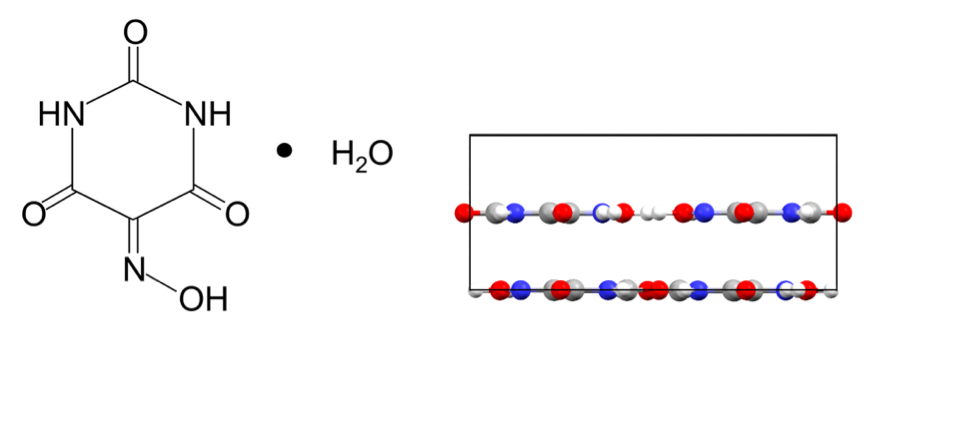
\includegraphics[width=1\linewidth]{src/figures/VAMH_figures/VAMH_fig1.png}
  \caption{A) Violuric acid monohydrate (VAMH) molecular structure and B) \textit{Cmc}2\textsubscript{1} crystal configuration. Viewed along c-axis.}
  \label{fig:vamh_fig}
\end{figure}

In a previous study we explored a proposed polymorphic phase transition of barbituric acid dihydrate, a structurally similar compound to VAMH. We concluded through experimental and computational analyses that the reported temperature-dependent phase transition was actually a result of thermal-induced crystal dynamic disorder and a relationship between a high-temperature disordered state and a low-temperature static state, both of which maintained the same crystal symmetry. The proposed phase transition occurred around 217 K, with the molecules shifting from a planar (\textit{Pnma}) to non-planar configuration (\textit{P}2\textsubscript{1}/n) as the temperature of the system was decreased \citep{nichol_btadh_2005,Jeffrey1961,Al-Karaghouli}. Our data was consistent with a dynamic crystal disorder resulting from the oscillation of two non-merohedrally twinned \textit{P}2\textsubscript{1}/n configurations. This oscillation was observed as a planar configuration by X-ray crystallography due to the average of the two energetically equivalent and closely spaced \textit{P}2\textsubscript{1}/n states. Due to the structural similarity between BTADH and VAMH, the accuracy of the VAMH planar \textit{Cmc}2\textsubscript{1}crystal structure was called into question \citep{paul_true_2019}.
Investigation into the crystal conformation of VAMH at 150 K concluded with a redetermination of the space group from planar \textit{Cmc}2\textsubscript{1}to non-planar \textit{Pca}2\textsubscript{1}. Initial normal-mode calculations of the \textit{Cmc}2\textsubscript{1}unit cell resulted in an imaginary mode. Relaxed symmetry geometry optimizations with the initial \textit{Cmc}2\textsubscript{1}unit cell parameters resulted in the perceived Z=2 unit cell with \textit{P}2\textsubscript{1} symmetry. Upon further analysis via THz spectrometry it was discovered that the simulated \textit{P}2\textsubscript{1} and experimental spectra showed poor agreement, with the number of calculated low-frequency phonon modes falling short of those observed experimentally. A final geometry optimization of a 2x2x2 supercell with \textit{P}\textsubscript{1} symmetry yielded a \textit{Pca}2\textsubscript{1} space group (Z=8). The simulated \textit{Pca}2\textsubscript{1} and experimental THz spectra displayed good alignment, concluding that the redetermined crystal structure of VAMH is of \textit{Pca}2\textsubscript{1} symmetry. 

\section{Materials and Methods}
\subsection{Experimental THz Measurements}
Samples were prepared for terahertz spectroscopy measurements by initially grinding a 2.5\% w/w mixture of violuric acid with polytetrafluoroethylene (PTFE) in order to homogenize the samples and reduce particle size in order to minimize scattering effects. The sample-PTFE mixture was then pressed into a free-standing 13mm diameter pellet using a hydraulic pellet press (Specac Ltd., UK), yielding an 888.34 mg pellet with a thickness of 3.03mm. A second pellet using only PTFE was used as a standard reference, with the same dimensions as the sample-containing pellet. The pellets were mounted in a closed-cycle liquid helium cryostat (Crycocool Industries, USA), which permitted variable temperature acquisition between 20 and 300 K. For the terahertz time-domain spectroscopy measurements, a commercial THz-TDS system (Toptica Photonics AG, DE) was used, which consists of a pair of fiber-coupled emitter and receiver modules. Four off-axis parabolic mirrors were used to collimate and focus the terahertz radiation, and the entire spectrometer was continuously purged with nitrogen gas to minimize absorption from atmospheric water vapor. At each temperature, 20,000 terahertz time-domain waveforms were averaged for both the sample and blank, which was repeated four times. The time-domain data were Fourier transformed to obtain terahertz power spectra, and each sample-blank pair was used to produce absorption spectra, with four absorption spectra per temperature averaged to yield the final spectra presented. 
\subsection{Solid-State Density Functional Theory}
The Crystal17 software package was utilized to perform all DFT calculations, using the PBE-D3 functional and pob-TZVP \citep{Peintinger2013} basis set combination \citep{Dovesi2017,Dovesi2014}. Default values were used for the three-body (D3) empirical energy correction for London-type dispersion forces \citep{Dovesi2017,Grimme2010,Grimme2011,Grimme2016}. Atom-only geometry optimizations were run on VAMH confined to the \textit{Cmc}2\textsubscript{1}space group. Initial lattice dimensions and atomic coordinates for this optimization were obtained from the Cambridge Crystallographic Database \cite{nichol_violuric_2005,groom_cambridge_2016}. Space group perceptions were performed using the Avogadro software package with atom position tolerances of 0.01 Å or less \citep{avogadro}. Constant volume geometry optimizations were performed with energy convergence criteria of \(\Delta\)E < 10-6 hartree for initial optimizations and \(\Delta\)E < 10\textsuperscript{-8} hartree for geometry optimizations used for frequency calculations. Normal mode calculations were run for the optimized structures using the total energy convergence criteria of \(\Delta\)E < 10\textsuperscript{-11} hartree. The optimal sampling rate for the k points used to defined the real space density matrix and the reciprocal space Monkhorst grid were determined for the total energy convergence of \(\Delta\)E < 10\textsuperscript{-11} hartree for the \textit{Cmc}2\textsubscript{1}optimization \citep{Gilat1972,monkhorst}. Shrinking factors of 6 were used for all calculations in order to meet the above listed energy convergence criteria. The radial and angular distributions of points were defined by a pruned (75,974) integration grid for each calculation. The truncation tolerances for the Coulomb and HF exchange integral series were set to 10\textsuperscript{-8}, 10\textsuperscript{-8}, 10\textsuperscript{-8}, 10\textsuperscript{-8}, and 10\textsuperscript{-16} hartree. The IR intensities for the normal mode calculations were determined by the Berry phase approach of calculating polarization differences between equilibrium and distorted geometries utilizing the dipole moment derivatives (d\(\mu\)/dQ) \citep{pascale_calculation_2004, Kudin2007,Wu1993}.

\section{Results and Discussion}
\par Initial geometry optimizations of VAMH were performed with the molecules confined to \textit{Cmc}2\textsubscript{1}symmetry group with fixed lattice parameters corresponding to the experimental X-ray crystal structure determined at 150 K (a = 6.0754 Å, b = 14.3430 Å, c = 7.5288 Å, Z = 4). The atomic coordinates from the \textit{Cmc}2\textsubscript{1}cell optimizations were used in a normal mode caluclation for VAMH, resulting in a single imaginary mode at -22.33 cm\textsuperscript{-1}. The potential energy surface following the imaginary mode displacements were scanned, resulting in a double-well potential, with a small energy barrier of 0.058 kJ mol\textsuperscript{-1} between the two energetically equivalent minima (\autoref{fig:vamh_doublewell}). Graphical representations of the displacement vectors for the imaginary mode were constructed to view the molecular displacements associated with the imaginary mode (\autoref{fig:vamh_imaginarymode}). As seen, the atomic displacements were observed to be equal, but opposite across the vertical mirror plane (parallel to the b-c plane) within the molecule, suggesting an in-phase rocking motion between two mirrored configurations.

\begin{figure}[htbp]
  \center
  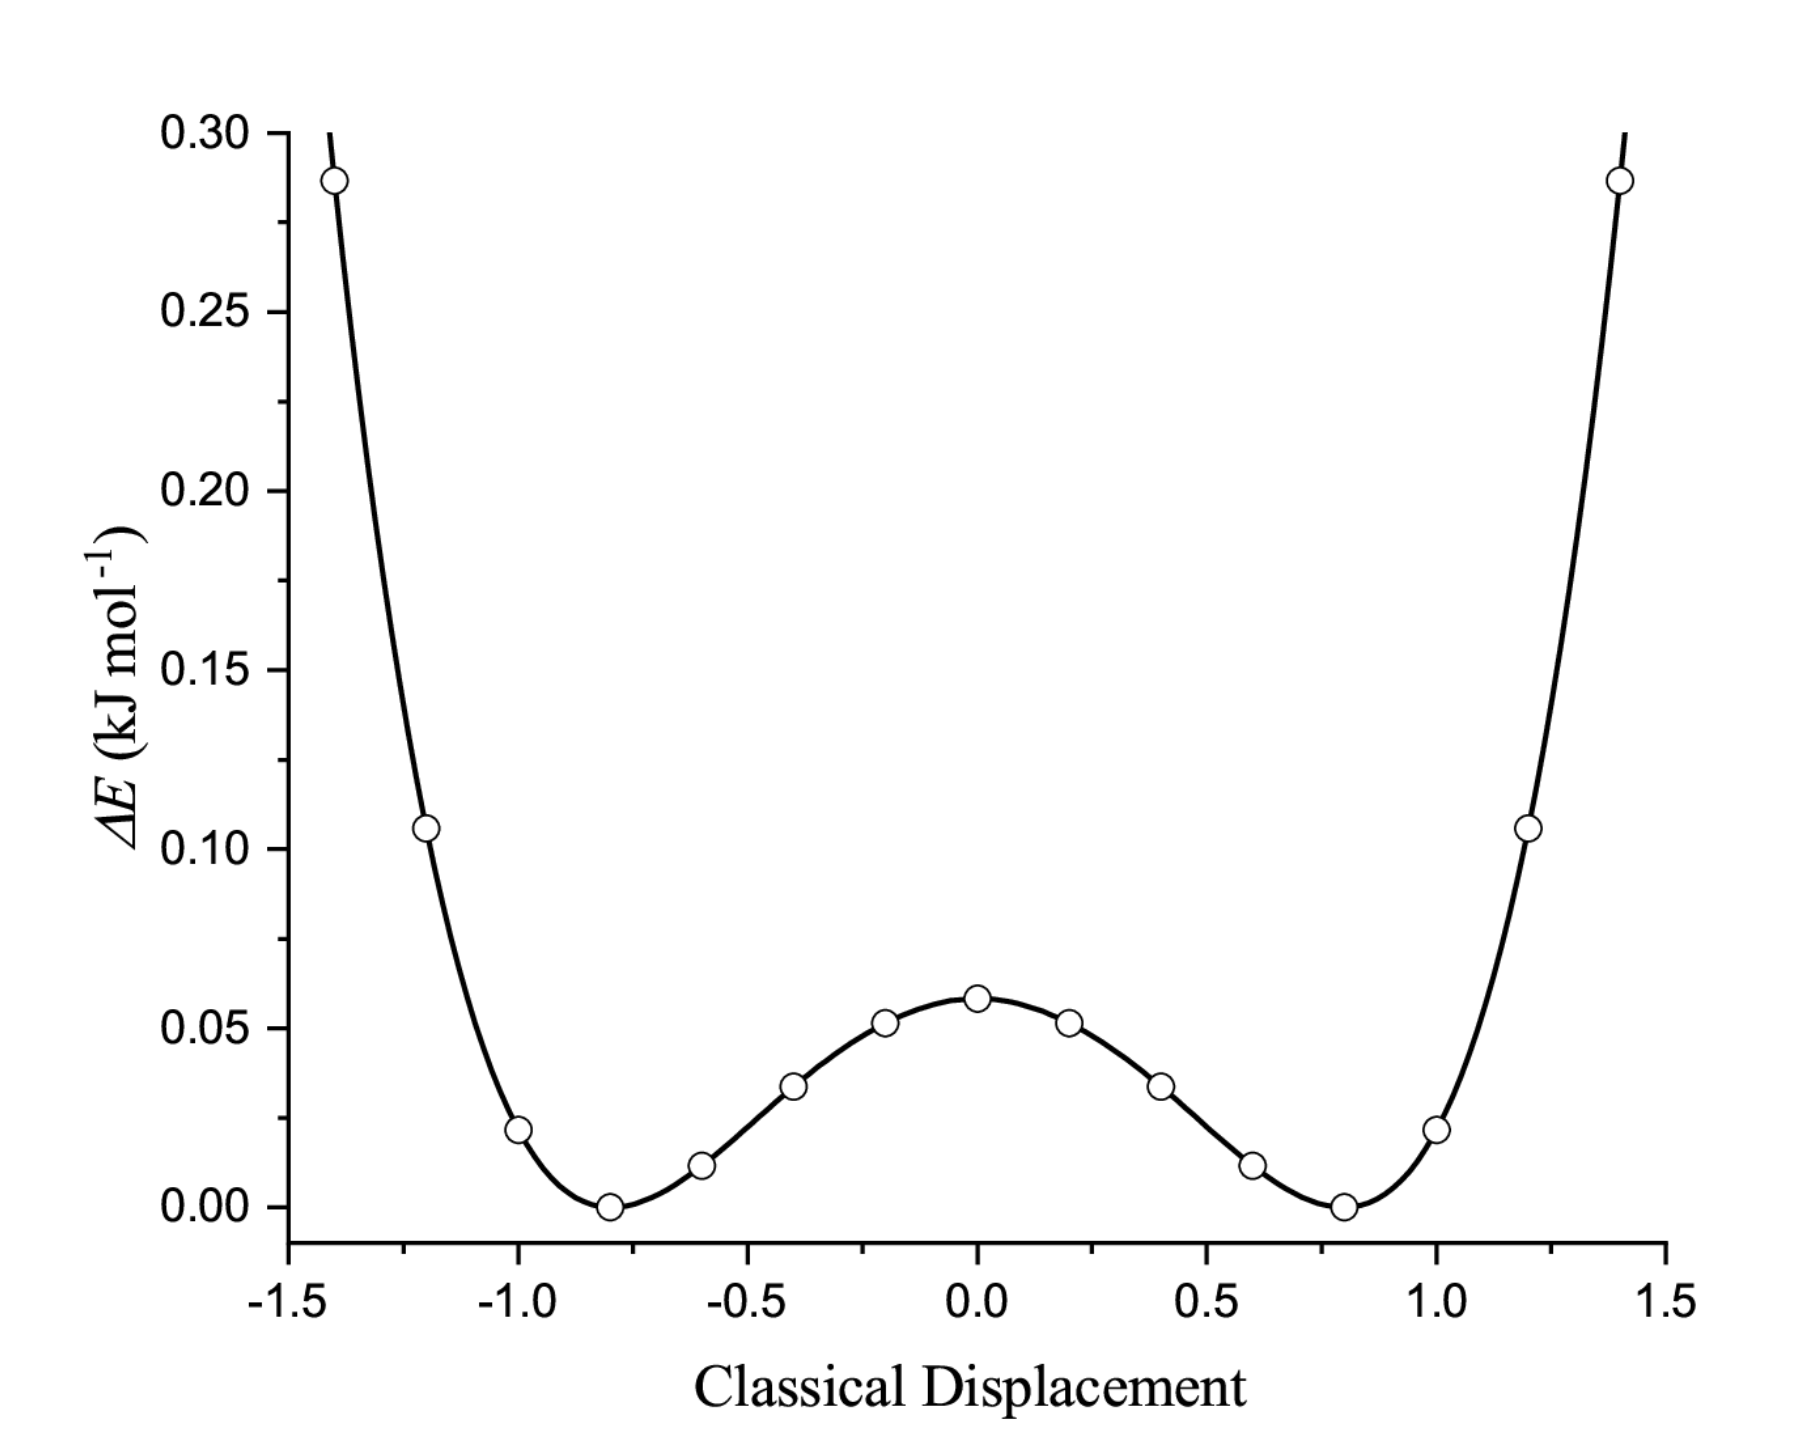
\includegraphics[width=1\linewidth]{src/figures/VAMH_figures/VAMH_potescan.png}
  \caption{Potential energy scan along imaginary mode at 150 K.}
  \label{fig:vamh_doublewell}
\end{figure}

\begin{figure}[ht]
  \center
  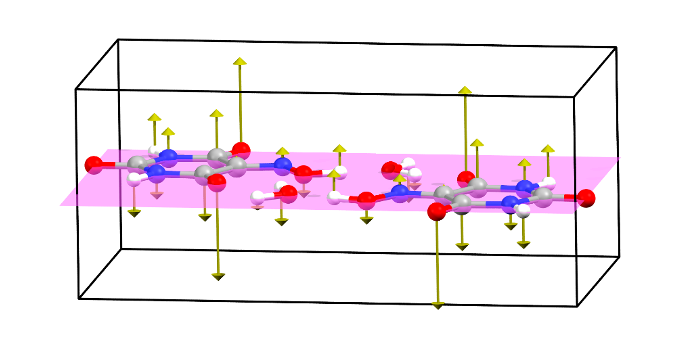
\includegraphics[width=1\linewidth]{src/figures/VAMH_figures/VAMH_fig3.png}
  \caption{A) Vibrational character of the imaginary mode clauclated at 22.33 cm-1 for VAMH constrained to \textit{Cmc}2\textsubscript{1}space group symmetry. Atomic displacement vectors are represented by yellow arrows (magnitudes scaled ×10). }
  \label{fig:vamh_imaginarymode}
\end{figure}

To further investigate the energetically favorable crystalline packing of VAMH, all symmetry constraints were removed, relaxing the \textit{Cmc}2\textsubscript{1}space group to \textit{P}\textsubscript{1}. Constant-volume geometry optimizations were performed at various volumes to investigate the effect of unit cell size (i.e. thermal expansion) on the optimization of the molecules. The lattice parameters and calculated electronic energies of the optimized structures are tabulated in the Supporting Informtion. The molecules in each of the resulting optimized structures were shifted slightly out of plane, as seen in \autoref{fig:vamh_p1andp21} and \autoref{vamh_planes}.  The optimized \textit{P}\textsubscript{1} structure corresponding to the 150-K experimental unit cell volume was analyzed, and a higher-symmetry \textit{P}2\textsubscript{1} molecular configuration was perceived with parameters a = 6.31442 Å, b = 7.31395 Å, c = 7.74019 Å, \(\beta\) = 113.4318°, Z = 2. The \textit{P}2\textsubscript{1} space group contained only two asymmetric units, which is a reduction of half from the original \textit{Cmc}2\textsubscript{1}space group. Subsequent constant volume geometry optimizations with \textit{P}2\textsubscript{1} symmetry were conducted resulting in the b-cell length being reduced by approximately half from the \textit{Cmc}2\textsubscript{1}to \textit{P}2\textsubscript{1} configuration, along with the \(\beta\)-angle increasing from 90° to approximately 113°. An overlay of the \textit{P}\textsubscript{1} (green) and \textit{P}2\textsubscript{1} (black) unit cells within the crystal structure is shown in \autoref{fig:vamh_p1andp21}A. 

\begin{figure}{ht!}
  \center
  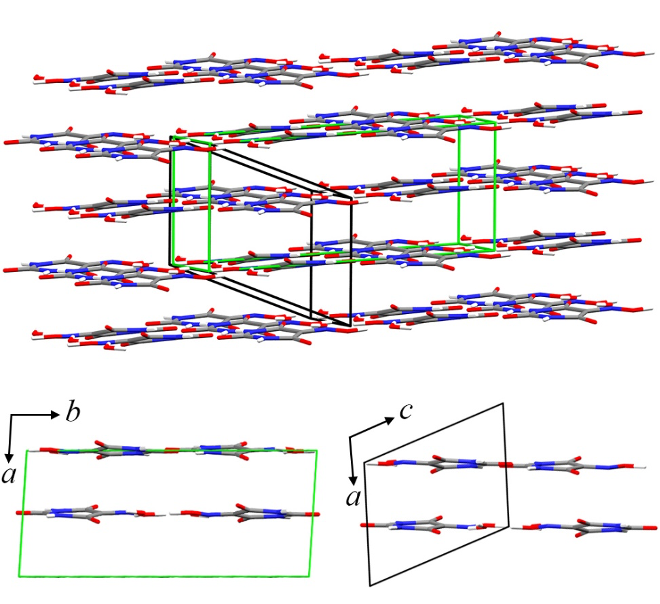
\includegraphics[width=1\linewidth]{src/figures/VAMH_figures/VAMH_fig4.png}
  \caption{A) \textit{P}\textsubscript{1} and \textit{P}2\textsubscript{1} unit cell overlay. B) Packed \textit{P}\textsubscript{1} unit cell viewed along the c axis. C) Packed \textit{P}2\textsubscript{1} unit cell viewed along the b axis.}
  \label{fig:vamh_p1andp21}
\end{figure}

\begin{figure}{ht!}
  \center
  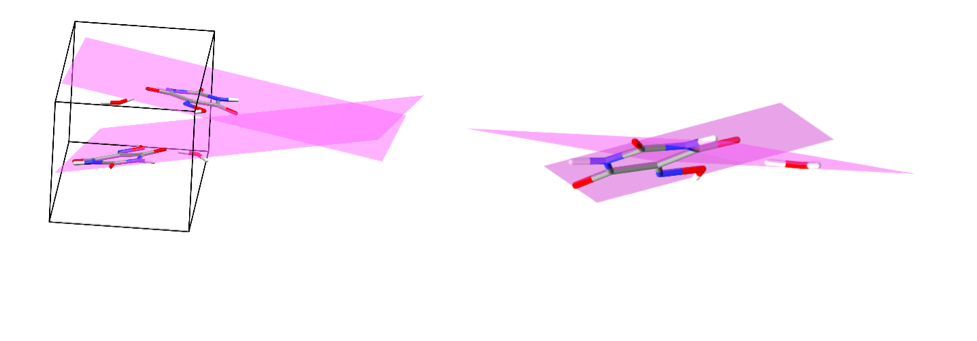
\includegraphics[width=1\linewidth]{src/figures/VAMH_figures/vamh_fig5.png}
  \caption{Depicted planes between A) violuric acid molecules and B) water violuric acid molecular planes of VAMH confined to the \textit{P}2\textsubscript{1} space group.}
  \label{vamh_planes}
\end{figure}


Correlating the static molecular orientations observed in the \textit{P}\textsubscript{1} and \textit{P}2\textsubscript{1} optimized structures with the imaginary mode character obtained from the \textit{Cmc}2\textsubscript{1}normal mode calculations revealed that the out-of-plane molecular shifts correspond to the direction of the imaginary mode displacement vectors shown in \autoref{vamh_planes}. This break in planar symmetry from \textit{Cmc}2\textsubscript{1}to \textit{P}2\textsubscript{1} can be explained by the changes in intermolecular contacts between the two configurations (\autoref{fig:vamh_electrostatic_contacts}, \autoref{tab:vamh_distances}). Relaxation of the crystal symmetry permits the formation of more stable hydrogen bonding and an increased distance of repulsive O···O contacts between adjacent VA molecules (labeled as contact 5). Considerably more favorable direct hydrogen bonding involving the water molecule was obtained in \textit{P}2\textsubscript{1}, most markedly for contact 2 which was reduced by -0.501 Å in comparison to the \textit{Cmc}2\textsubscript{1}structure. Contacts 1 and 4 were modestly reduced by -0.033 and -0.028 Å, respectively. The contact 3 distance remained relatively unchanged between the two crystal structures. Also contributing to the addition stabilization of the \textit{P}2\textsubscript{1} optimized structure is the increase in the short-contact O···O distance between carbonyl oxygens of neighboring VA molecules by 0.048 Å, thereby reducing the repulsive strain forces present within the crystal structure.

\begin{figure}[ht!]
  \center
  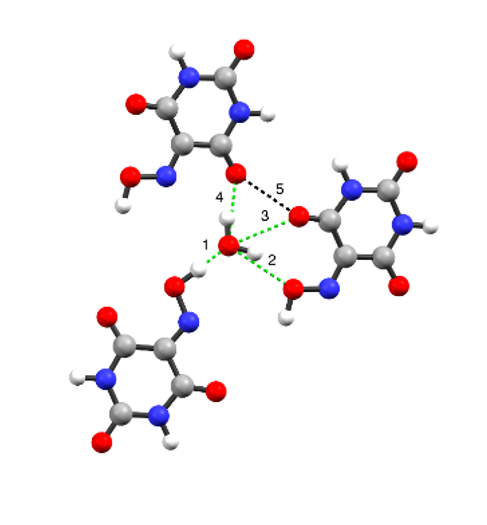
\includegraphics[width=0.7\linewidth]{src/figures/VAMH_figures/VAMH_fig6.png}
  \caption{Primary electrostatic contacts observed in the VAMH crystal structures. Hydrogen bonds are indicated by dashed green lines and repulsive interactions by dashed black lines.}
  \label{fig:vamh_electrostatic_contacts}
\end{figure}

\begin{table}[h]
    \centering
    \caption{Heavy atom distances for intermolecular contacts observed in the \textit{Cmc}2\textsubscript{1}and \textit{P}2\textsubscript{1} optimized unit cells.}
    \begin{tabular}{cccc}
    & \multicolumn{2}{c}{\textbf{Distance (Å)}} & \\
    \textbf{Contact} & \textbf{Cmc2\textsubscript{1}} & \textbf{\textit{P}2\textsubscript{1}} & \textbf{Difference} \\
    \hline
    \textit{1} & 2.507 & 2.474 & -0.033 \\
    \textit{2} & 2.969 & 2.468 & -0.501 \\
    \textit{3} & 2.758 & 2.761 & 0.003 \\
    \textit{4} & 2.676 & 2.648 & -0.028 \\
    \textit{5} & 2.745 & 2.793 & 0.048 \\
    \end{tabular}
    \label{tab:vamh_distances}
\end{table}

In effort to validate the proposed \textit{P}2\textsubscript{1} symmetry configuration of VAHM, the phonon vibrational frequecnies were calculated using the optimized crystal coordinates. As expected, there were no imaginary modes calculated in the normal mode analysis of the \textit{P}2\textsubscript{1} crystal structure, suggesting that a minimum energy configuration was acchieved. The calculated low-frequency vibrational modes were subsequently compared to experiemtnal THz spectrum of VAMH obtained in the spectral range of 10-130 cm-1 (\autoref{vamh_p21_thz}). It was observed that the simulated \textit{P}2\textsubscript{1} THz spectra did not align well with the experimental spectrum, with a notably lower claculated density of states. Only 5 IR-active phonon modes having appreciable absorption intensities were claulcted in the probed spectral range while 9 modes could clearly b resolved in the experimental THz spectrum, along with several evident underlying modes contributing to obsereved peak asymmetry. The additional peaks in the experimental spectrum could not be accounted for with the predicted \textit{P}2\textsubscript{1} crystal structure, however the calculated modes could be tentatively correlated to observed spectral features. This inducated that the basic VAMH molecular orientations predicted in the \textit{P}2\textsubscript{1} configuration were perhaps correct, but the Z=2 unit cell was too reduced and thereby limited the number of phonon modes present in the calculations. 

\begin{figure}[ht!]
  \center
  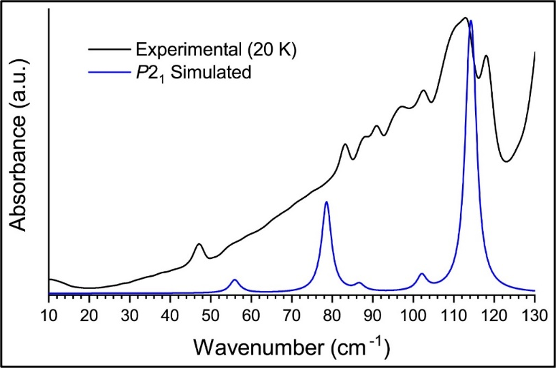
\includegraphics[width=1\linewidth]{src/figures/VAMH_figures/vamh_fig7.png}
  \caption{Comparison of the simulated \textit{P}2\textsubscript{1} THz spectrum to the experimental THz spectrum obtained at 20 K. Lorentzian lineshapes of FWHM 5 cm-1 were convolved into calculated normal modes, and mode intensities of calculated and experimental spectra were normalized.}
  \label{vamh_p21_thz}
\end{figure}

In light of the information provided by the experimental THz spectra, a 2×2×2 supercell was generated from the original \textit{Cmc}2\textsubscript{1}crystal structure, and a geometry optimization was performed with reduced \textit{P}\textsubscript{1} symmetry under constant volume constraints. The resulting structure was then analyzed for symmetry elements present winthin the \textit{P}\textsubscript{1} supercell. Using an atomic-position tolerance of 0.05 Å, a new unit cell of \textit{Pca}2\textsubscript{1} symmetry was percieved to be contained within the optimized \textit{P}\textsubscript{1} supercell structure (\autoref{fig:vamh_pca21}). The VAMH molecular orientations of the larger \textit{Pca}2\textsubscript{1} (Z=8, Z’=2) resembled those observed in the previously predicted \textit{P}2\textsubscript{1} (Z=2, Z’=1) crystal structure. However, the VAMH molecular pairings along the elongated c axis were now related by a screw axis as opposed to restricted translationally invariant in the reduced \textit{P}2\textsubscript{1} packing configuration. The predicted lattice demensions of the \textit{Pca}2\textsubscript{1} and the \textit{P}2\textsubscript{1} crystal structures provided in \autoref{tab:vamh_unitcell_params}. 

\begin{figure}[ht!]
  \center
  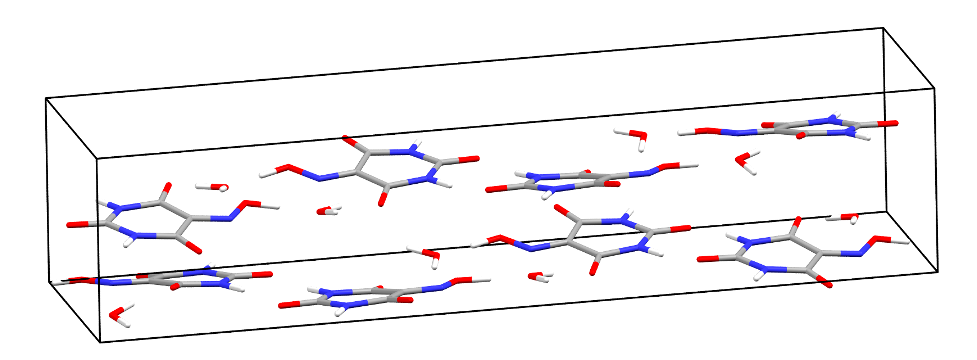
\includegraphics[width=1\linewidth]{src/figures/VAMH_figures/vamh_fig8.png}
  \caption{Molecular packing of the predicted VAMH \textit{Pca}2\textsubscript{1} crystal structure.}
  \label{fig:vamh_pca21}
\end{figure}
  
Comparison of calculated unit cell energies shows the energetic favorability of the \textit{Pca}2\textsubscript{1} unit cell configuration, with relative energy 1.052 kJ mol-1 molecule-1 lower in energy than the \textit{P}2\textsubscript{1} cell and 1.647 kJ mol-1 molecule-1 lower than the constrained \textit{Cmc}2\textsubscript{1}structure (\autoref{tab:vamh_unitcell_params}). The energy difference separating each crystal form is small and presents a low transition barrier between equivalent configurations related by the \textit{Cmc}2\textsubscript{1}reflection planes. The phase coexistence is likely the cause of the apparent crystal disorder and the original conclusion of VAMH residing in the \textit{Cmc}2\textsubscript{1}space group, as this would represent the average of two mirrored equivalent energetic minima. 


\begin{table}[h]
    \centering
    \caption{Tabulated comparison of the unit cell parameters and electronic energies of the investigated symmetry groups.}
    \begin{tabular}{cccccc}
    &&&&& \textbf{Relative Energies} \\
    & \textbf{a (Å)}& \textbf{b (Å)}& \textbf{c (Å)}& \textbf{beta (\textsuperscript{o}) }& \textbf{(kJ mol-1 molecule-1)}\textsuperscript{a}\\
    \hline
    \textsuperscript{b}\textbf{Cmc2\textsubscript{1}} & 6.0754 & 14.3430 & 7.5288 & 90 & 1.647 \\
    \textbf{\textit{P}2\textsubscript{1}}	& 6.31442 & 7.31395 & 7.74019 & 113.4318 & 1.052 \\
    \textbf{\textit{Pca}2\textsubscript{1}} & 7.32092 & 6.31631 & 28.37480 & 90 & 0.000 \\
    \hline
    \multicolumn{6}{l}{\textsuperscript{a}Relative energies obtained from constant-volume optimizations; \textsuperscript{b}Ref \citep{nichol_violuric_2005}.}
    \end{tabular}
    \label{tab:vamh_unitcell_params}
\end{table}

Normal modes of vibration were calculated for the predicted \textit{Pca}2\textsubscript{1} crystal structure and the low-frequency vibrational modes were compared with the experimental THz spectrum (\autoref{fig:vamh_pca21_thz}). A good quality fit of the simulated spectrum to the experimental was obtained. The number of calculated modes is sufficient to assign many of the experimental peaks, with additional low-intensity calculated modes that likely contribute to the high and uneven baseline of the THz spectrum, as well as to the peak asymmetry observed in several of the experimental features. The calculated vibrational frequencies were generally underestimated upon inspection of the spectral comparison. A reasonable explanation for this result is the comparison of the simulated spectrum calculated from an effective 150 K unit cell volume s the structure was optimized under constant-volume conditions from the original \textit{Cmc}2\textsubscript{1}crystal structure measured at this temperature \citep{leguy_dynamic_2016}. The simulated spectrum is overlayed with the experimental spectrum obtained at 20 K for enhanced resolution of experimental spectral features.  
 
\begin{figure}[ht!]
  \center
  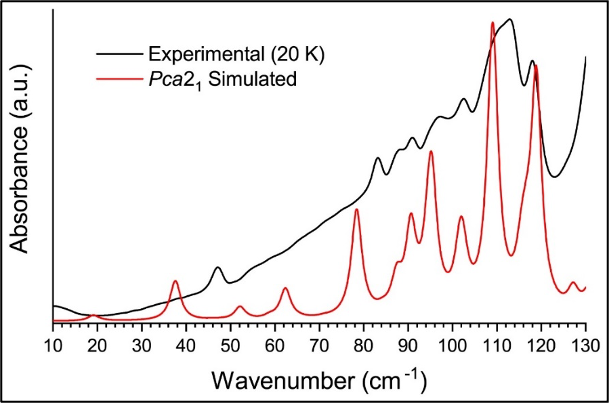
\includegraphics[width=1\linewidth]{src/figures/VAMH_figures/vamh_fig9.png}
  \caption{Comparison of the simulated \textit{Pca}2\textsubscript{1} THz spectrum to the experimental THz spectrum obtained at 20 K. Lorentzian lineshapes of FWHM 5 cm\textsuperscript{-1} were convolved into calculated normal modes, and mode intensities of calculated and experimental spectra were normalized. }
  \label{fig:vamh_pca21_thz}
\end{figure}

Through a systematic computational analysis of the VAMH crystal structure in conjuction with experimental validation by low-frequency THz spectroscopy, a redetermination of the VAMH crystal structure was achieved. The previously reported \textit{Cmc}2\textsubscript{1} crystal structure exhibiting a planar arrangement of violuric acid and water molecules was shown to be inaccurate and likely the result of structural averaging during experimental X-ray measurements. Similar behavior was previously reported for the structurally similar barbituric acid dihydrate, for which a planar configuration  of \textit{Pnma} symmetry was reported for the suspected low-temperature polymorph. However, it was conclusively demonstrated that the crystal structure maintained \textit{P}2\textsubscript{1}/n symmetry, that which was reported as the high-temperature polymorph. In the cases of both VAMH and barbituric acid dihydrate, the planar crystalline configuration represents an averaged structure at the transition point connecting two symmetry-equivalent mirrored unit cell structures. At the two minima, distinct crystal symmetries exist that do not conform to the reflection planes imposed by the \textit{Cmc}2\textsubscript{1}and \textit{Pnma} space groups, respectively. In the present study, a more energetically favorable configuration of \textit{Pca}2\textsubscript{1} was identified for VAMH. The validity of the predicted structure was verified using THz spectroscopy. Normal mode calculations of the optimized \textit{Pca}2\textsubscript{1} crystal structure produced phonon modes that were in good agreement with the experimental THz spectra. 

\section{Conclusion}
Investigation into the crystal structure of VAMH demostrated the theoretical and experimetal data did not support the proposed \textit{Cmc}2\textsubscript{1}symmetry configuration. Imaginary modes were observed across a broad range of defined unit cell volumes while VAMH was confined to the planar \textit{Cmc}2\textsubscript{1}configuration. Initial geometry optimizations with all symmetry operations removed resulted in a perceived Z=2 unit cell of space group \textit{P}2\textsubscript{1}. The shift in molecular orientation was supported by the plotting of the displacement vectors along the observed imaginary mode. This information supported that the actual crystalline arrangement of VAMH deviated from the planar configuration, and that the planar structure may be the averaged structure connecting two energetically equivalent non-planer structures. Explained by the double-well potential and imaginary modes revealed with VAMH confined to the \textit{Cmc}2\textsubscript{1}space group. However, when the simulated THz spectrum of the \textit{P}2\textsubscript{1} unit cell was compared to the experimentally obtained spectrum, there was poor agreement between the two. Further evaluation of the original crystal structure yielded an orthorhomic \textit{Pca}2\textsubscript{1} space group configuration following the generation and structural optimization of a 2x2x2 supercell (Z=32) in \textit{P}\textsubscript{1} symmetry. The normal-mode calculation for the \textit{Pca}2\textsubscript{1} unit cell resulted in no imaginary modes and nearly harmonic potentials for the low-frequency phonon modes. When comparing the simulated \textit{Pca}2\textsubscript{1} and experimental THz spectra, there was good alignment between theory and experiment. This study provides a conclusive redetermination of the violuric acid monohydrate crystal structure in \textit{Pca}2\textsubscript{1} symmetry.
